\documentclass[addpoints,spanish, 12pt,a4paper,cancelspace]{./include/gexam}

%%%%%%%%%%%%%%%%%%%%%%%%%%%
\renewcommand{\documentName} { Recuperación final junio }
\renewcommand{\documentContent} { Todas las evaluaciones } 
\renewcommand{\waterMark} { \phantom{Modelo A} } 

% Configuración del documento.
\renewcommand{\schoolSubject} { Examen Matemáticas 2º ESO  }
\renewcommand{\school} { IES José de Churriguera  }
\renewcommand{\academicPeriod} { Curso 2022/2023 }

\renewcommand{\autor} { Andrés Giménez Muñoz }
\renewcommand{\emailAuthor} { andresprofemates@outlook.es }
\renewcommand{\autorSing}{ Profesor: Andrés } 
%%%%%%%%%%%%%%%%%%%%%%%%%%%

%%%%%%%%%%%%%%%%%%%%%%%%%%%
% Exam configuration
%\pointsdroppedatright   %% No mostrar la puntuación
\pointsinrightmargin % Para poner las puntuaciones a la derecha. Se puede cambiar. Si se comenta, sale a la izquierda.
\extrawidth{-1.5cm} %Un poquito más de margen por si ponemos textos largos.
\marginpointname{ \emph{\points}}

%% Si se comenta no aparecerán los espacios de la solución.
%\nocancelspace

%% Esto es de la clase exam. Si dejamos sin comentar \printanswers, se mostraran las soluciones. 
%% Si la comentamos y dejamos sin comentar \noprintanswers, pues no se muestran las soluciones.
%\printanswers
%\noprintanswers

%%%%%%%%%%%%%%%%%%%%%%%%%%%

\begin{document}

\StudentData
\GradeTableHeader

\justifying

\begin{center}
    \fbox{\fbox{\parbox{6.5in}{             
                \begin{itemize}
                    \item Copiar, hablar, levantarse de la silla o molestar al resto de la clase pueden ser motivos de la retirada del examen que se valorará con un cero.
                    \item Deben aparecer todas las operaciones, no vale solo con indicar el resultado.
                    \item Se podrán quitar hasta cinco décimas por falta de claridad o rigor en el desarrollo de las respuestas o por una mala presentación.
                    % \item Se valorará que se indiquen las cuentas en línea, realizando las operaciones en el margen.
                    \item Está permitido utilizar la calculadora.
                \end{itemize}
            }}}
\end{center}

\begin{questions}
    \setcounter{question}{0}

    \question[2] Calcula:
        \begin {parts}
            \part $2\cdot 3^2-\frac{4^2}{2}+3^2-\left(-1\right)^4=$
            \vspace{\stretch{1}}
            \part $20 + \left[3 \cdot 4 - \left(17- 3 \cdot 2^2 \right) \right] \cdot 2 =$
            \vspace{\stretch{1}}
            
            % \part
            % $\frac{(\frac{2}{3})^5 \cdot (\frac{2}{3})^0 \cdot (\frac{2}{3})^{-3}}
            %     {\left(\frac{3}{2}\right)^{-5} \cdot \left(\frac{2}{3}\right) \cdot \left[\left(\frac{2}{3}\right)^5 \right]^2}=$
            % \vspace{\stretch{1}}
            % \newpage{}

            \part
            $\left(\frac{2}{3}-\frac{4}{5}\right):\frac{7}{15}+\left(1+\frac{1}{2}-\frac{11}{14}\right) = $
            \vspace{\stretch{1}}

            % \part
            % $\left(\sqrt[10]{5^2}\right)^5 + \sqrt[4]{16} = $
            % \vspace{\stretch{1}}
        \end{parts}

    % \question[1] Rellena el cuadro
    % \begin{table}[h]
    %     \centering
    %     \renewcommand{\arraystretch}{2}

    %     \begin{tabular}{|p{5cm}|p{3cm}|m{5cm}|}
    %         \hline
    %         \rowcolor[gray]{.9}
    %         \textbf{Representación gráfica} & \textbf{Intervalos} & \textbf{Definición matemática} \\ \hline
    %         & \multicolumn{1}{c|}{$[-1, 3)$}     &                       \\ [0.4cm] \hline
    %         \center \tikz\draw [*-o] (0,0) node[pos=2, below] {$-2$} -- +(3,0) node[pos=1, below] {$4$}; &          &              \\ [0.4cm] \hline 
    %                    &         & \multicolumn{1}{c|}{$\left\{x | x > 0 \right\}$}  \\ [0.4cm] \hline
    %         \center \tikz\draw [<-*] (0,0) node[pos=2, below] {$-\infty$} -- +(3,0) node[pos=1, below] {$3$};&      &               \\ [0.4cm] \hline
    %     \end{tabular}
    % \end{table}

    \newpage{}
    \question Resuelve los siguientes problemas
    \begin {parts}
        \part[1] Entre tres hermanos deben repartirse 12 \euro{}. 
        El primero se lleva $\sfrac{7}{16}$ del total, el segundo $\sfrac{5}{12}$ del total y el tercero el resto. 
        ¿Qué fracción del total se lleva el 3º? 
        ¿Cuánto dinero se ha llevado cada uno?
        \vspace{\stretch{1}}
        
        \part[1]
        La población de una pequeña ciudad según antiguo censo era de 560 habitantes. 
        Se ha realizado un nuevo censo y los datos informan de un incremento del $7\%$.
        ¿Cuál es la población actual?  
        \vspace{\stretch{1}}

        % \part[1]
        % Cinco amigos que van de excursión y gastan 850\euro{} en 10 días. ¿Cuánto gastarán 8 personas en 12 días? 
        % \vspace{\stretch{1}}

        % \part[1]
        % Tres estudiantes participan en un concurso para repartirse el premio de 240\euro{} de forma inversamente proporcional al número de errores cometidos.
        % El primero alumno cometió 8 errores, el segundo 6 errores y el tercero 3 errores. 
        % ¿Cuánto recibirá cada uno? 
        % \vspace{\stretch{2}}
    \end{parts}

    \newpage{}

    \question[2]
    Siendo $P(x) = 3x^4-4x^2+3x$, $Q(x)=-2x^3-x^2+x-2$, $R(x)=x^2-2$, calcula:
    \begin {parts}
        \part $Q(-1)$
        \vspace{\stretch{2}}
        % \part $P(x) - Q(x)$
        % \vspace{\stretch{1}}
        % \part $P(x):R(x)$
        % \vspace{\stretch{1}}
        \part $P(x) \cdot Q(x)$
        \vspace{\stretch{2}}
    \end{parts}

    \question[2]
    Resuelve el sistema de ecuaciones por el método que consideres más adecuado e indica el nombre del método utilizado:
    \begin{parts}
        \part
        % Por el método de sustitución:
        \begin{flushleft}
            $\begin{cases}
                    \nonumber
                    2x - y  = 1 \\
                    \nonumber
                    -4x + y = 25
                \end{cases}$
        \end{flushleft}
        \vspace{\stretch{3}}

        % \part
        % Por el método de igualación.
        % \begin{flushleft}
        %     $\begin{cases}
        %             \nonumber
        %             -3x - 4y = 5 \\
        %             \nonumber
        %             -2x + 3y = 9
        %         \end{cases}$
        % \end{flushleft}
        % \vspace{\stretch{1}}

        % \part
        % % Por el método de reducción.
        % \begin{flushleft}
        %     $\begin{cases}
        %             \nonumber
        %             2x + 3y = 1 \\
        %             \nonumber
        %             x + y = -2
        %         \end{cases}$
        % \end{flushleft}
        % \vspace{\stretch{1}}
    \end{parts}

    % \newpage

    % \question[2]
    % Resuelve el siguiente sistema de ecuaciones por el método gráfico.
    % \begin{flushleft}
    %     $\begin{cases}
    %             \nonumber
    %             2x + 3y  = 14 \\
    %             \nonumber
    %             -x + 2y = 0
    %         \end{cases}$
    % \end{flushleft}

    % \begin{figure}[h]
    %     \centering
    %     \begin{subfigure}[b]{0.4\textwidth}
    %         \begin{tabular}{|w{c}{1cm}|w{c}{1cm}|}
    %             \multicolumn{2}{c}{$ 2x + 3y  = 14 $}   \\ \hline
    %             x & y \\ \hline
    %             &   \\
    %             &   \\
    %             &   \\
    %             &   \\
    %             &   \\
    %             &   \\
    %             &   \\ \hline
    %         \end{tabular}        \end{subfigure}
    %     \begin{subfigure}[b]{0.4\textwidth}
    %         \begin{tabular}{|w{c}{1cm}|w{c}{1cm}|}
    %             \multicolumn{2}{c}{$ -x + 2y = 0 $}   \\ \hline
    %             x & y \\ \hline
    %             &   \\
    %             &   \\
    %             &   \\
    %             &   \\
    %             &   \\
    %             &   \\
    %             &   \\ \hline
    %         \end{tabular}
    %     \end{subfigure}
    % \end{figure}

    % \vspace{\stretch{1}}

    % \begin{figure}[h]
    %     \centering
    %     \begin{tikzpicture}[scale=0.7]
    %         \tkzInit[xmax=10,ymax=10,xmin=-10, ymin=-10]
    %         \tkzGrid[color=black!50]
    %         \tkzAxeXY
    %     \end{tikzpicture}
    % \end{figure}

    % \newpage
    % \question[2]
    % Resuelve las siguientes ecuaciones:
    % \begin{parts}
    %     % \part
    %     % $-(-2x-1)-3(x+5)=x+12$
    %     % \vspace{\stretch{1}}

    %     \part
    %     $\frac{x-3}{2}-\frac{3x-5}{2} = -1$
    %     \vspace{\stretch{1}}

    %     \part
    %     $x-13=4\left[3x-4\left(x-2\right)\right]$
    %     \vspace{\stretch{1}}
    % \end{parts}

    % \newpage

    % \question[3]
    % Resuelve las siguientes ecuaciones de segundo y tercer grado
    % \begin{parts}
    %     \part 
    %     $(x-2) (x+2) (x-3) = 0$
    %     \vspace{\stretch{1}}

    %     \part 
    %     $3x^2+3x=2x^2$
    %     \vspace{\stretch{1}}

    %     \part 
    %     $x^2+x-6=0$
    %     \vspace{\stretch{1}}

    % \end{parts}

    \newpage
    \question[2] Obtén la ecuación de la recta que pasa por los puntos A(5,4) y B(6,2) 
    expresándola en su forma general y explicita y represéntala en el eje de coordenadas.

    \vspace{\stretch{1}}

    % \begin{figure}[h]
    %     \centering
    %     \begin{tikzpicture}[scale=0.5]
    %         \tkzInit[xmax=10,ymax=10,xmin=-10, ymin=-10]
    %         \tkzGrid[color=black!50]
    %         \tkzAxeXY
    %     \end{tikzpicture}
    % \end{figure}


    \begin{center}
        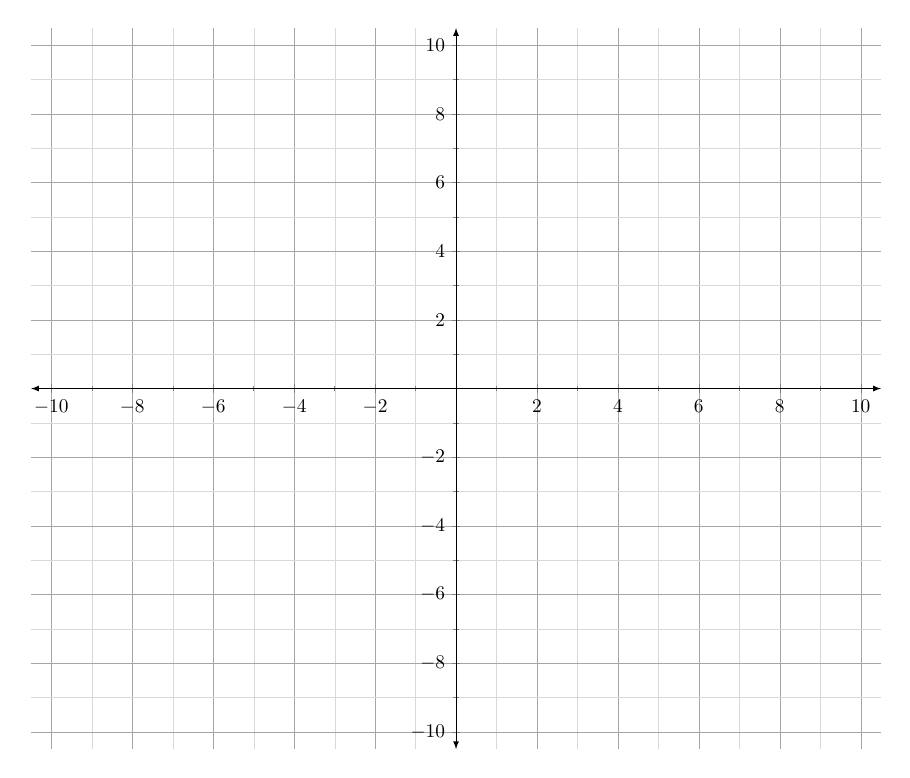
\begin{tikzpicture}[scale=0.7]
            \begin{axis}[
                axis x line=center,
                axis y line=center,
                xmin=-10,xmax=10,
                ymin=-10,ymax=10,
                grid=both,
                grid style={line width=.1pt, draw=gray!30},
                major grid style={line width=.2pt,draw=gray!70},
                axis lines=middle,
                axis line style={<->},
                minor tick num=1,
                enlargelimits={abs=0.5},
                axis line style={latex-latex},
                % ticklabel style={font=\tiny,fill=white},
                % xlabel style={at={(ticklabel* cs:1)},anchor=north west},
                % ylabel style={at={(ticklabel* cs:1)},anchor=south west},
                xlabel style={below right},
                ylabel style={above left},
                width=17cm,
            ]
        \end{axis}
        \end{tikzpicture}
    \end{center}

    % \newpage

    % \question[3] Dada la parábola $y = x^2 - 3x + 2$ calcula su vértice, punto de corte con los ejes de coordenadas 
    % e indica si el vértice es un máximo o un mínimo.
    % \vspace{\stretch{1}}
    
    % \begin{center}
    %     \begin{tikzpicture}[scale=0.7]
    %         \begin{axis}[
    %             axis x line=center,
    %             axis y line=center,
    %             xmin=-10,xmax=10,
    %             ymin=-10,ymax=10,
    %             grid=both,
    %             grid style={line width=.1pt, draw=gray!30},
    %             major grid style={line width=.2pt,draw=gray!70},
    %             axis lines=middle,
    %             axis line style={<->},
    %             minor tick num=1,
    %             enlargelimits={abs=0.5},
    %             axis line style={latex-latex},
    %             % ticklabel style={font=\tiny,fill=white},
    %             % xlabel style={at={(ticklabel* cs:1)},anchor=north west},
    %             % ylabel style={at={(ticklabel* cs:1)},anchor=south west},
    %             xlabel style={below right},
    %             ylabel style={above left},
    %             width=17cm,
    %         ]
    %     \end{axis}
    %     \end{tikzpicture}
    % \end{center}

    % \newpage
    % \question[3] En un momento determinado del día la sombra de Juan mide $2,50m$ y la de un arbol $35m$, 
    % sabiendo que Juan mide $1,75m$ ¿cuál es la altura del arbol?
    % \\ \\
    % \begin{minipage}{\linewidth}
    %     % \centering
    %     \includegraphics[width=7cm]{img01}
    % \end{minipage}
    % \vspace{\stretch{1}}

    % \newpage 
    % \question[1] Al dar una vuelta completa a la rueda de una bicicleta, está avanza $2,83m$ ¿Cuánto milímetros mide el diámetro de la rueda?
    % \\ \\
    % \begin{minipage}{\linewidth}
    %     % \centering
    %     \includegraphics[width=7cm]{img02}
    % \end{minipage}
    % \vspace{\stretch{1}}

\end{questions}
\end{document}